\chapter{Mobiele HTML5 raamwerken}
\label{chap:mobiele-html5-raamwerken}
In dit hoofdstuk gaan we inzoomen op bestaande mobiele HTML5 raamwerken die gebruik maken van de laatste nieuwe technologieën zoals HTML5, CSS3 en JavaScript. Deze raamwerken worden gecategoriseerd volgens twee courante aanpakken~\cite{Oeflman2011}: opmaak-up gedreven en JavaScript gedreven. Bij een opmaak-up gedreven aanpak wordt de webapplicatie voornamelijk in HTML code geschreven. Daarentegen wordt bij een JavaScript gedreven aanpak hoofdzakelijk in JavaScript geprogrammeerd.

\section{jQuery Mobile}
jQuery Mobile is een mobiel HTML5 \term{user interface} (UI) raamwerk dat werd aangekondigd in 2010~\cite{Resig2010}. In november 2011 werd versie 1.0 uitgebracht~\cite{Parker2011} en een jaar later werd in oktober versie 1.2 uitgebracht~\cite{Parker2012}. Op het moment van schrijven kwam versie 1.3 uit~\cite{Parker2013a}. Het raamwerk wordt beheerd door het jQuery Project dat onder andere jQuery Core beheert en waar jQuery Mobile afhankelijk van is~\cite{JQuery2012}. jQuery Mobile wordt door onder andere Adobe, BlackBerry en Mozilla gesponsord~\cite{JQuery2012a}.

\subsection{Omkadering}
\paragraph{Programmeertaal}
Om met jQuery Mobile aan de slag te kunnen, heb je niets meer nodig dan kennis over HTML, CSS en JavaScript. Alle UI elementen worden geschreven in HTML en aangeduid met \code{data-}* attributen.

\paragraph{Tools}
Een basis teksteditor voldoet om met jQuery Mobile aan de slag te kunnen. Natuurlijk kan het gemakkelijk zijn om van \term{integrated development environments}~(IDE's) zoals Aptana Studio~\cite{Aptana2012} of WebStorm~\cite{JetBrains2012} gebruik te maken, waardoor je handige kenmerken krijgt zoals \term{code completion}.

Je kan ook gebruiken maken van Codiqua om via \term{drag-and-drop} UI elementen op je scherm te slepen. Codiqua zal automatisch op de achtergrond de HTML code voorzien~\cite{Sperry2012}.

\paragraph{Documentatie}
Documentatie is te vinden op \url{www.jquerymobile.com/demos/1.2.0}. Hierop is een catalogus te vinden van alle mogelijke elementen waarover jQuery Mobile beschikt. Door de broncode van een voorbeeld te bekijken, kan je zien welke code je moet schrijven om tot dat resultaat te komen.

Naast de UI elementen is er ook documentatie over de API. Deze gaat over initiële configuraties, events en methodes die kunnen worden gebruikt.

% \paragraph{Community}
% Met 7.400 volgers op GitHub~\cite{GitHub2012} en 11.200 volgers op Twitter~\cite{Twitter2012} komt de grote kracht van jQuery Mobile van zijn community . Dit heeft grotendeels te maken met het feit dat jQuery Mobile geniet van het succes van jQuery, dat ook zeer populair is~\cite{Hales2012}.
%TODO Sander: dit komt in de vergelijkingscriteria

\paragraph{Marktadoptatie}
Als we kijken op de website van jQuery Mobile zien we een reeks applicaties gemaakt met hun raamwerk. Enkele voorbeelden zijn webapplicaties voor Ikea, Disney World, Stanford University en Moulin Rouge~\cite{JQuery2012a}. 

\paragraph{Licenties}
Vanaf september 2012 is het enkel nog mogelijk om jQuery Mobile onder de Massachusetts Institute of Technology (MIT) licentie te verkrijgen~\cite{Dmethvin2012}. Dit betekent dat de code wordt vrijgegeven als \term{open-source} en dat deze tegelijkertijd kan worden gebruikt in propriëtaire projecten en applicaties~\cite{PhilDutson2012}.

\subsection{Code en ontwikkeling}
Zoals werd aangehaald, schrijft men vooral HTML5 code voorzien van \code{data-}* attributen. Daarna zal het raamwerk door middel van \term{progressive enhancement} allerhande code toevoegen om de beoogde UI elementen correct te tonen in de browser. Dit wordt verder uitgelegd in de sectie browserondersteuning (zie \ref{sec:jqm-browser-support}).

Er zijn drie strategieën om webapplicaties te maken in jQuery Mobile~\cite{Broulik2012}. Een eerste is om de volledige applicatie in één webpagina te schrijven. Met andere woorden,  de vele schermen van de webapplicatie zijn dan allemaal samengebracht op eenzelfde webpagina. Het voordeel bij deze aanpak is dat er initieel minder verzoeken zijn naar de server omdat alles in één bestand wordt opgehaald. Dit geldt ook zo voor de geïmporteerde CSS en JavaScript-bestanden. 

Een tweede strategie is om voor ieder scherm een aparte webpagina aan te maken. Het voordeel hierbij is dat de eerste pagina waar de gebruiker op terecht komt, sneller wordt gedownload. Bij iedere navigatie naar een ander scherm, moet dit scherm via AJAX worden opgehaald, waardoor dit vertragend kan werken. 

Een laatste strategie is om een mix tussen beide te maken. Men kan bijvoorbeeld alle schermen die de gebruiker vaak nodig heeft op één webpagina plaatsen. De schermen die de gebruiker zelden nodig heeft, plaats men dan op aparte webpagina's.  

\subsection{Functionele kenmerken}
jQuery Mobile is een raamwerk dat voornamelijk UI elementen aanbied, met name pagina's en dialoogvensters, werkbalken, knoppen, inhoud vormgeven, elementen voor formulieren en lijsten~\cite{JQuery2012b}.

\paragraph{Pagina's en dialoogvensters}
De basisstructuur van een pagina bestaat uit een koptekst, inhoud en voettekst. Bij het overgaan naar een andere pagina kan men kiezen uit tien overgangseffecten. Voordat deze overgang gebeurt, zal jQuery Mobile altijd eerst die pagina ophalen via AJAX en inladen in het DOM. Zo kan een soepel overgangseffect worden getoond aan de gebruiker. Daarnaast is het ook mogelijk om gelinkte pagina's op voorhand op te halen. Als laatste biedt jQuery Mobile ook dialoogvensters en pop-ups aan. 

\paragraph{Werkbalken}
Het is mogelijk om zowel knoppen bij de koptekst als bij de voettekst te plaatsen. Bij deze laatste kunnen typisch meer knoppen geplaatst worden, bij de koptekst slechts twee. Daarnaast is het ook mogelijk om navigatiebalken te maken. Aan zowel de werk- als navigatiebalken kunnen iconen worden toegevoegd.

\paragraph{Knoppen}
Het is ook mogelijk om knoppen te plaatsen in het inhoud gedeelde. Ook hier is er terug een variëteit aan mogelijkheden: grote of kleine, met iconen of zonder, gegroepeerd of niet. 

\paragraph{Inhoud vormgeven}
De inhoud van de pagina kan worden vormgegeven door gebruik te maken van een rooster. jQuery Mobile laat roosters tot vijf kolommen toe. Daarnaast zijn er ook nog opklapbare blokken ter beschikking. Als laatste kunnen deze blokken ook samengevoegd worden tot een accordeon. 

\paragraph{Elementen voor formulieren}
jQuery Mobile biedt alle gangbare elementen voor formulieren aan zoals textinvoer, een selectie uit een lijst, een zoekveld, een \term{slider} en een \term{switch}. Het raamwerk verplicht zelf om de \code{<label>}-tag te gebruiken. Zo wordt de applicatie toegankelijker gemaakt voor bijvoorbeeld mensen met een \term{e-reader}.

\paragraph{Lijsten}
Een laatste categorie UI elementen die jQuery Mobile aanbiedt, zijn lijsten. Deze gaan van standaard ongeordende lijsten tot lijsten met alle soorten decoraties als iconen, afbeeldingen, telbubbels en verdelers. Ook is het mogelijk om in deze lijsten te zoeken. Hiervoor dient de gebruiker enkel één data attribuut toe te voegen, waarna het raamwerk de implementatie voorziet. 

\subsection{Niet-functionele kenmerken}
\paragraph{Performantie}
Zoals gezegd schrijft de ontwikkelaar HTML5 code met specifieke data attributen en zal het raamwerk daarna de code verder aanvullen. Dit gebeurt enkel op de pagina die de gebruiker op dat moment bekijkt. Dit gaat dus ook op voor een webapplicatie waarbij alle schermen op één webpagina zijn geschreven. Deze webpagina bevat allemaal \code{<div>}-verpakkingen voor ieder scherm. jQuery Mobile zal enkel die \code{<div>} verder aanvullen die op dat moment getoond wordt aan de gebruiker. 

\paragraph{Aanpasbaarheid}
Als je jQuery Mobile \term{out-of-the-box} gebruikt, zit alles al goed qua kleur en design. Je hebt de keuze uit vijf kleurenthema's die je kan toepassen op de gehele applicatie of enkel op bepaalde elementen. Om je applicatie echt te laten onderscheiden van de andere, zal je natuurlijk graag je eigen kleurthema willen toepassen. Hier is jQuery Mobile op voorzien door hun \term{stylesheet} op te delen in twee delen: thema's en structuur. Je kan als ontwikkelaar ook enkel de structuur downloaden en zelf de thema CSS schrijven. Daar dit laatste heel wat inspanning vraagt, hebben de ontwikkelaars van jQuery Mobile ook een tool ter beschikking,  namelijk ThemeRoller~\cite{JQuery2012c}. Hier kan je zeer eenvoudig kleuren slepen naar een voorbeeldapplicatie. Eenmaal tevreden kan je de overeenkomstige \term{stylesheet} downloaden en toevoegen aan je project.

\paragraph{Programmeerbaarheid}
Bij het programmeren in jQuery Mobile wordt geen enkel ontwerppatroon afgedwongen. De code voor de UI elementen wordt tenslotte als HTML5 code geschreven. Voor de echte functionaliteit wordt beroep gedaan op JavaScript en meer bepaald op de jQuery Core bibliotheek. Ook deze dwingt geen ontwerppatroon af.

% TODO deze tekst zal later moeten worden verplaatst
Een ander raamwerk, genaamd The-M-Project~\cite{Panacoda2012}, dwingt het Model-View-Controller (MVC) echter wel af. Met dit raamwerk is het mogelijk om webapplicaties te maken die het jQuery Mobile raamwerk gebruiken. In plaats van HTML5-code te schrijven, zoals dat bij jQuery Mobile gebeurt, schrijft je JavaScript-code. The-M-Project zal dan zelf intern deze JavaScript-code omzetten naar de desbetreffende jQuery Mobile HTML5-code.

\paragraph{Browserondersteuning}
\label{sec:jqm-browser-support}
jQuery Mobile deelt browsers op in drie verschillende klassen: A, B en C~\cite{JQuery2012d}. Hierbij ondersteunt een klasse A browser alles, terwijl een klasse C browser enkel de basis HTML ondersteunt (en dus bijvoorbeeld geen hippe CCS3 overgangen).

Er dient een onderscheid te worden gemaakt tussen de begrippen \emph{progressive enhancement} en \emph{graceful degradation}~\cite{Hens2012}. Het eerste is wat jQuery Mobile toepast, namelijk starten met de basis HTML. Deze code wordt door iedere browser, dus ook deze uit de C klasse, op een goede manier weergegeven. Daarna zal het iteratief elementen toevoegen tot het op een moment komt dat de betreffende browser een bepaald kenmerk niet meer ondersteund.

De tegenhanger is \emph{graceful degradation}. Hierbij wordt eerst een versie ontwikkeld die enkel in de meest recentste browser kan worden getoond. Daarna, als de ontwikkelaar nog tijd heeft, gaat hij \term{fallbacks} implementeren waardoor minder recente browser de applicatie ook kunnen weergeven.
%TODO Sander: is het niet nuttiger om progresive enhancement en graceful degration in Kenmerken detecteren en opvullen te bespreken?  jQuery gebruikt enkel progressive enhancement en kan dan verwijzen naar een vorige sectie..

%%%%%%%%%%%%%%%%%%%%%%%%%%%%%%%%%%%%%%%%%%%%%%%%%%%%%%%%%%%%%%%%%%
%%%%%%%%%%%%%%%%%%%%%%%%%%%%%%%%%%%%%%%%%%%%%%%%%%%%%%%%%%%%%%%%%%

\section{Sencha Touch}

Sencha Touch is een relatief verschillend raamwerk in vergelijking met jQuery Mobile.  Het wordt ontwikkeld door Sencha,  een bedrijf dat in 2010 is ontstaan als een samensmelting van Ext JS,  jQuery Touch en Raphaël.  Ext JS is een JavaScript raamwerk voor de ontwikkeling van web applicaties. jQuery Touch is een jQuery plugin voor mobiele web ontwikkeling.  Het steunt op WebKit en voegt \term{touch events} toe aan jQuery.  Raphaël,  ten slotte,  is een JavaScript bibliotheek voor vector tekeningen. Op het moment van schrijven is Sencha Touch aan versie 2.1.1~\cite{Inc.}.  

\subsection{Omkadering}
\paragraph{Programmeertaal}
Sencha Touch is JavaScript gedreven dus all functionaliteiten worden in JavaScript geïmplementeerd. Het aanroepen van het raamwerk gebeurt door het invoeren van de Sencha Touch bibliotheek binnen \code{<script>}-elementen.  Alle HTML code wordt bij het bekijken van de pagina gegenereerd.  

\paragraph{Tools}
Naast Sencha Touch levert Sencha nog producten die Sencha Touch uitbreiden of het leven van de ontwikkelaar makkelijker maken.  Deze worden hieronder opgelijst~\cite{Inc.}.  

\subparagraph{Sencha Animator}
Dit is een desktop applicatie om CSS3 animaties te ontwerpen.  Deze animaties worden enkel in WebKit browsers ondersteund.

\subparagraph{Sencha Architect}
Dit is een andere desktop applicatie waarmee je makkelijk een UI kan ontwikkelen met behulp van \term{drag-and-drop} commando's.  

\subparagraph{Sencha GXT}
Sencha GXT is een uitbreiding op Google Web Toolkit (GWT).  De compiler van GWT laat toe applicaties in Java te schrijven en ze te compileren naar geoptimaliseerde,  \term{cross-browser} HTML5 en JavaScript.  Sencha GXT voegt grafieken,  widgets, etc. toe aan GWT.

\subparagraph{Sencha.IO}
Deze uitbreiding zorgt voor \term{cloud} services binnen mobiele applicaties.  

\paragraph{Documentatie}
Alle documentatie voor Sencha Touch 2.1.1 is te vinden op \url{docs.sencha.com/touch/2-0}.  Een zoekfunctie voor objecten,  eigenschappen en methoden is aanwezig om snel zaken op te zoeken.  De meeste functionaliteiten zijn voorzien van codevoorbeelden samen met het resultaat hoe de browser de code rendert.  Verder biedt de Sencha website ook een groot aanbod om Sencha te leren gebruiken \url{www.sencha.com/learn/touch/}.  Hier staan handleidingen,  introductie video etc..

%Door de snelle ontwikkeling van Sencha blijft de documentatie niet altijd up-to-date.  Zo zijn vele methoden verouderd maar staat er geen alternatief vermeld. 
%TODO dit is misschien eerer subjectief?
Een ander handig raadslagwerk is de ‘Kitchen Sink'~\cite{Inc.2013}.  Dit is een webapplicatie,  geschreven in Sencha Touch,  die de belangrijkste functionaliteiten bevat samen met de bijhorende code.  


% \paragraph{Community}
% We kunnen vaststellen dat Sencha over een grote community beschikt.  Met meer dan 2 miljoen ontwikkelaars wereldwijd is Sencha de grootste provider van een open-source web applicatie~\cite{Inc.}.  

\paragraph{Marktadoptatie}
Volgens de Sencha website is 50\% van de Fortune 100 - een lijst van de grootste Amerikaanse bedrijven gerangschikt op jaaromzet - een Sencha klant~\cite{Inc.}.  Enkele van hun grootste klanten zijn CNN,  Samsung,  Cisco en  Visa.

\paragraph{Licenties}
Sencha Touch is gratis binnen een commerciële context waarbij het bedrijf in kwestie de broncode niet deelt voor zijn gebruikers.  Wanneer je dit wel wil doen bestaat er ook een gratis \term{open-source} versie van Sencha Touch.  Deze komt met een GNU GPL v3 \term{open-source} licentie wat wil zeggen dat je de vrijheid hebt om aanpassingen aan de broncode te maken en te verspreiden,  zolang je zelf je code maar gratis verspreid voor alle gebruikers.
  
Voor de ontwikkeling van eigen raamwerken of SDKs betaal je een \term{original equipment manufacturer} (OEM) licentie.  Dit wil zeggen dat bedrijven hun producten gaan verkopen onder hun eigen merk en naam, maar gebruik maken van Sencha.  Omdat het gebruik hiervan per gebruiker verschilt,  worden OEM licenties op maat gemaakt~\cite{Inc.}.

\subsection{Code en ontwikkeling}
Zoals reeds vermeld moet alle code in JavaScript worden geschreven en dient één HTML bestand slechts als container om de bestanden in te laden.  Sencha valt dus onder JavaScript gebaseerde raamwerken.  De keuze voor deze aanpak heeft twee belangrijke motivaties.  Enerzijds is Sencha Touch gebouwd op Ext JS,  wat op zich een JavaScript raamwerk is.  Anderzijds zorgt het voor een betere ondersteuning voor toestellen met verschillende resoluties.  Samen met SASS en Compass kan Sencha lay-outs definiëren per device (zie sectie \ref{sec:sencha-aanpasbaarheid}).  De \code{Ext.env.Browser} en \code{Ext.env.OS} eigenschappen en \code{Ext.Viewport.getOrientation} en \code{Ext.feature.has} methoden kunnen de vereisten bepalen en de juiste lay-out kiezen~\cite{JohnEClark2012}.

Om het de ontwikkelaars makkelijker te maken biedt Sencha ook SDK tools aan.  Momenteel bevinden deze zich nog in bèta.  Concreet zijn deze tools commando's voor de terminal die onder andere nieuwe projecten kunnen aanmaken, JavaScript bestanden kunnen optimaliseren maar vooral de webapplicatie kunnen omzetten naar native applicaties voor iOS en Android.

\paragraph{Debugging}
Het debuggen van je code gebeurt voornamelijk in de browser zelf.  Tools als de Safari Web Inspector,  Chrome Developer Tools of Firebug moeten de fouten kunnen opsporen.  De broncode van Sencha Touch kan ook ingeladen worden met \code{sencha-touch-debug.js} als bibliotheek.  Deze versie is niet gecomprimeerd en bevat commentaar en documentatie om makkelijker te zoeken waar in de code de fout zich juist bevond.

\subsection{Functionele kenmerken}
Net zoals jQuery Mobile heeft Sencha Touch ook een hele hoop functionaliteiten om eenvoudig UI elementen te genereren.  Sencha Touch bevat alle elementen van de UI als JavaScript objecten.  Net zoals alle objectgerichte programmeertalen maken deze objecten gebruik van een klassesysteem,  iets wat slechts vanaf Sencha Touch 2 werd ingevoerd.  Op die manier kunnen klassen worden gedefinieerd (\code{Ext.define}) en aangemaakt (\code{Ext.create}).  Hierbij is ook overerving mogelijk.  De basisklasse van alle objecten is \code{Ext.Component}.  Componenten kunnen gerenderd worden, zichzelf tonen of verbergen,  centreren op het scherm en zichzelf aan- of uitzetten.   Het aanmaken van componenten kan compacter door het gewenste component als \code{xtype} te definiëren.  

Een andere belangrijke component is \code{Ext.Container}.  Containers kunnen subcomponenten bevatten en een lay-out specifiëren.  Alle componenten krijgen een naam die verwijst naar een namespace.  Dit is handig om conflicten te vermijden tussen je eigen objecten en de standaard objecten van het raamwerk.  

Voor een opsomming van alle raamwerk compontenten verwijzen we naar de documentatie~\cite{Inc.2013a}.

%jQuery subsecties:
%Pagina's en dialoogvensters
%werkbalken
%knoppen
%inhoud vormgeven
%elementen voor formulieren
%lijsten

\paragraph{Model}
Data kan intern worden voorgesteld met models.  Dit is iets wat hoort bij het MVC patroon (zie sectie \ref{sec:sencha-programeerbaarheid}).  Een model specifieert een lijst van velden die bij het model horen waarbij een veld een naam en een type heeft.  Optioneel kunnen validaties bij de velden worden toegevoegd om data consistent te houden.  

\paragraph{Store}
\code{Ext.data.Store} is de klasse om instanties van een model op te slaan.  Een \term{store} wordt voorzien van een \term{proxy}.  Deze kan data aan de client of server zijde opslaan.  Een \term{proxy} voor opslag aan client zijde kan zowel in het RAM geheugen als in de \term{local storage} van de browser opslaan.  Een \term{proxy} voor server opslag kan data verzenden via AJAX (zelfde domein) of JSONP (verschillende domeinen).  Een \term{proxy} kan ook nog voorzien worden van een \term{reader} die aangeeft hoe de ontvangen data gelezen moet worden.

\paragraph{View}
Een \term{view} is de benaming voor objecten die aan de gebruiker kunnen getoond worden.  Een voorbeeld hiervan zijn lijsten,  waar vaak de data van een \term{store} wordt in weergegeven.  Zo'n lijst kan makkelijk gefilterd of gesorteerd worden op basis van velden uit het model.  Hiervoor moeten we \term{filters} of \term{sorters} aan de \term{store} toevoegen.  De lay-out van één lijstitem bepalen kan via een \code{XTemplate}.  Het sjabloon bepaalt de HTML structuur van elk item.  Alle gedefinieerde velden van het model kunnen in de template worden opgeroepen of gemanipuleerd.

\subsection{Niet-functionele kenmerken}
\paragraph{Performantie}
In vergelijking met versie 1.1 van Sencha Touch is de performantie gestegen om wille van verschillende factoren.  De introductie van het klasse systeem,  zoals besproken in de vorige sectie,  laat toe objecten dynamisch te laden.  Het grote verschil tussen \code{Ext.define} en \code{Ext.create} is dat objecten enkel in het geheugen worden geladen na creatie.  Het is dus de taak van de programmeur om objecten enkel te construeren wanneer ze nodig zijn.

Verder kwam versie 2.0 met een nieuwe lay-out \term{engine} die vooral het verwisselen van oriëntatie van het toestel versnelde.  Ook een verbetering in performantie op Android toestellen,  voornamelijk bij scrollen en animaties,  werd ingevoerd~\cite{Inc.}.

Een benchmark voor deze verbeteringen zijn de opstarttijden van de Kitchen Sink applicatie.  Het opstarten gebeurde met de verschillende Sencha Touch versies en op verschillende toestellen.  De resultaten zijn terug te vinden op figuur \ref{fig:sencha_performance}.  Op bijna elk toestel blijkt Sencha Touch 2.0 ongeveer één seconde sneller te werken~\cite{SenchaInc.2013}.

\begin{figure}
  \centering
  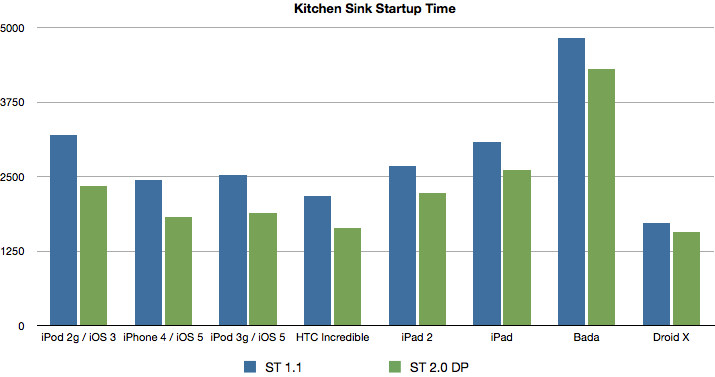
\includegraphics[width=0.8\textwidth]{figuren/sencha-touch-startup-times.png}
  \caption{Sencha Touch Kitchen Sink opstarttijden~\cite{SenchaInc.2013}.}
  \label{fig:sencha_performance}
\end{figure}

\paragraph{Aanpasbaarheid}
\label{sec:sencha-aanpasbaarheid}
Elke component binnen het raamwerk moet overerven van \code{Ext.Component}.  Deze voorziet een attribuut \code{ui}.  De waarde hiervan is een CSS klasse die bepaald hoe de component er zal uitzien.  Sencha heeft al twee CSS klassen voorzien:  \code{light} en \code{dark}.  Andere componenten kunnen deze lijst uitbreiden.  Een knop kan bijvoorbeeld \code{normal},  \code{back},  \code{round},  \code{small},  \code{action} of \code{forward} als \code{ui} waarde hebben.

Het is ook mogelijk om eigen waarden voor \code{ui} te definiëren of de standaarden van Sencha aan te passen.  Hiervoor moet je gebruik maken van SASS en Compass om je CSS bestanden aan te maken.  SASS staat voor Syntactically Awesome Stylesheets en breidt CSS uit met variabelen,  geneste structuren,  mixins en overerving~\cite{Eppstein2013}.  Mixins groeperen enkele CSS eigenschappen en kunnen worden herbruikt.  Compass is een raamwerk bovenop SASS en CSS.  Het compileert SCSS (Sassy CSS) naar CSS bestanden~\cite{Eppstein2013a}.        

Sencha thema's bestaan allemaal uit een set van mixins.  Door zelf mixins te creëren of reeds bestaande te manipuleren kunnen we eigen thema's creëren en ze aan de \code{ui}-waarde van een component toekennen.

\paragraph{Programmeerbaarheid}
\label{sec:sencha-programeerbaarheid}
Zoals reeds aangehaald ondersteund Sencha Touch het MVC (Model-View-Controller) patroon.  Dit patroon vermijdt lange JavaScript bestanden door ze logisch op te delen.  Modellen groeperen velden tot een beschrijving van data-objecten,  views definiëren de weergave van componenten en controllers verbinden beide op basis van events.

In theorie zou het verschil tussen mobiele websites en applicaties enkel in de views terug te vinden zijn.  Echter,  dit wordt nog niet volledig ondersteund en raadt men dus aan om hiervoor aparte projecten te voorzien.

\paragraph{Ondersteuning browser}
Sencha Touch steunt op de WebKit browser \term{engine} dus moet de browser deze bevatten.  Hoewel dit bij de meeste browsers geen probleem meer vormt vallen toch enkele populaire browsers uit de boot.  Sencha Touch is bijvoorbeeld niet compatibel met FireFox Mobile en Opera Mobile~\cite{JohnEClark2012}.

Zoals reeds vermeld zijn er ook methoden voorzien om informatie op te vragen over de context die gehanteerd wordt (browser, OS, toestel, etc.).  Verder kan Sencha Touch ook vragen naar de ondersteuning van specifieke kenmerken (audio,  canvas,  CSS3, …),  analoog als Modernizr.  

Op de Secha website zijn voor sommige browsers en bijhorend besturingssystemen scorecards voorzien om hun compatibiliteit met HTLM5 en Sencha Touch te bespreken~\cite{Inc.}.